\documentclass{scrartcl}
\usepackage[utf8]{inputenc}
\usepackage[T1]{fontenc}      
\usepackage[francais]{babel}
% Layout and figures
%\usepackage[top=2.5cm,bottom=2.5cm,right=2.5cm,left=2.5cm]{geometry}
\usepackage{subfigure}
\usepackage{rotating}
% Units and numbers
\usepackage[squaren, Gray]{SIunits}
\usepackage{sistyle}
\usepackage[autolanguage]{numprint}
% Math
\usepackage{amsmath}
\usepackage{amssymb}
\usepackage{amsthm}
% Links
\usepackage{url}
\usepackage{hyperref}
\hypersetup{
    colorlinks,
    citecolor=black,
    filecolor=black,
    linkcolor=black,
    urlcolor=black
}
% New commands
\newcommand{\annexe}{\part{Annexes}\appendix}
\newcommand{\biblio}[1]{\bibliographystyle{plain}\bibliography{#1}\nocite{*}}

\newcommand{\doctitle}[1]{
	\title{LSINF1225 - Projet BarTender}
	\subtitle{#1}
	\author{\textbf{Groupe T}\\
	\textsc{Gérard} Louis (6317-12-00)\\
	\textsc{Gillon} Bastien (5937-12-00)\\
	\textsc{Jacques} Thibault (0000-13-00)\\
	\textsc{Paris} Antoine (3158-13-00)\\
	\textsc{Ramelot} Sylvain (4763-13-00)}
	\date{\today}

	\begin{document}

	\maketitle
	%\tableofcontents
}

\doctitle{Partie 1 : ORM}
\section{Entités et faits élémentaires}
Dans un bar, on distingue plusieurs \textit{entités}.
On a avant tout le \textbf{client} et le \textbf{serveur}, qui
constituent les ``utilisateurs'' (aussi bien du bar que de
l'application). On a ensuite, la commande, la table et l'addition.
Enfin, on a une entité \textit{avis} qui représente l'avis (optionnel)
d'un client sur une boisson (cfr. extension ``ratings'').

Passons maintenant aux faits élémentaires pour chacune
de ces entités. Sur base de ces faits élémentaires, nous pourrons
ensuite établir un diagramme ORM (section \ref{sec:orm} 
ainsi qu'un population (section \ref{sec:population})
pour vérifier la validité de ce dernier.

\paragraph{Serveur}
\begin{itemize}
	\item Un serveur possède un login ;
	\item Un serveur possède un mot de passe ;
	\item Un serveur possède un nom ;
	\item Un serveur prend des commandes.
\end{itemize}

\paragraph{Client}
\begin{itemize}
	\item Un client possède un login ;
	\item Un client est assis à une table ;
	\item Un client possède un mot de passe ;
	\item Un client peut donner son avis.
\end{itemize}

\paragraph{Boisson}
\begin{itemize}
	\item Une boisson possède une description ;
	\item Une boisson possède un prix ;
 	\item Une boisson possède un nom ;
	\item Une boisson possède un volume ;
	\item Une boisson possède une quantité en stock ;
	\item Une boisson possède un ID ;
	\item Une boisson possède une icône ;
	\item Une boisson possède un stock seuil ;
	\item Une boisson possède un stock maximum ;
	\item Une boisson appartient à une catégorie ;
	\item Une boisson possède une sous-catégorie.
\end{itemize}

\paragraph{Commande}
\begin{itemize}
	\item Une commande est passée par une table ;
	\item Une commande est prise par un serveur ;
	\item Une commande est liée à une addition ;
	\item Une commande est associée à des boissons ;
	\item Une commande possède à un numéro de commande ;
	\item Une commande possède une date et une heure ;
	\item Une commande possède des quantités de boissons.
\end{itemize}

\paragraph{Table}
\begin{itemize}
	\item Une table accueille des clients ;
	\item Une table passe des commandes ;
	\item Une table possède un numéro de table.
\end{itemize}

\paragraph{Addition}
\begin{itemize}
	\item Une addition possède une date/heure ;
	\item Une addition possède un numéro d’addition ;
	\item Une addition comprend des commandes.
\end{itemize}

\paragraph{Avis}
\begin{itemize}
	\item Un avis est associé à une boisson ;
	\item Un avis contient une cote sur 5 ;
	\item Un avis peut contenir un commentaire ;
	\item L'avis est donné par un client.
\end{itemize}

\section{Diagramme ORM}
\label{sec:orm}
\rotatebox{90}{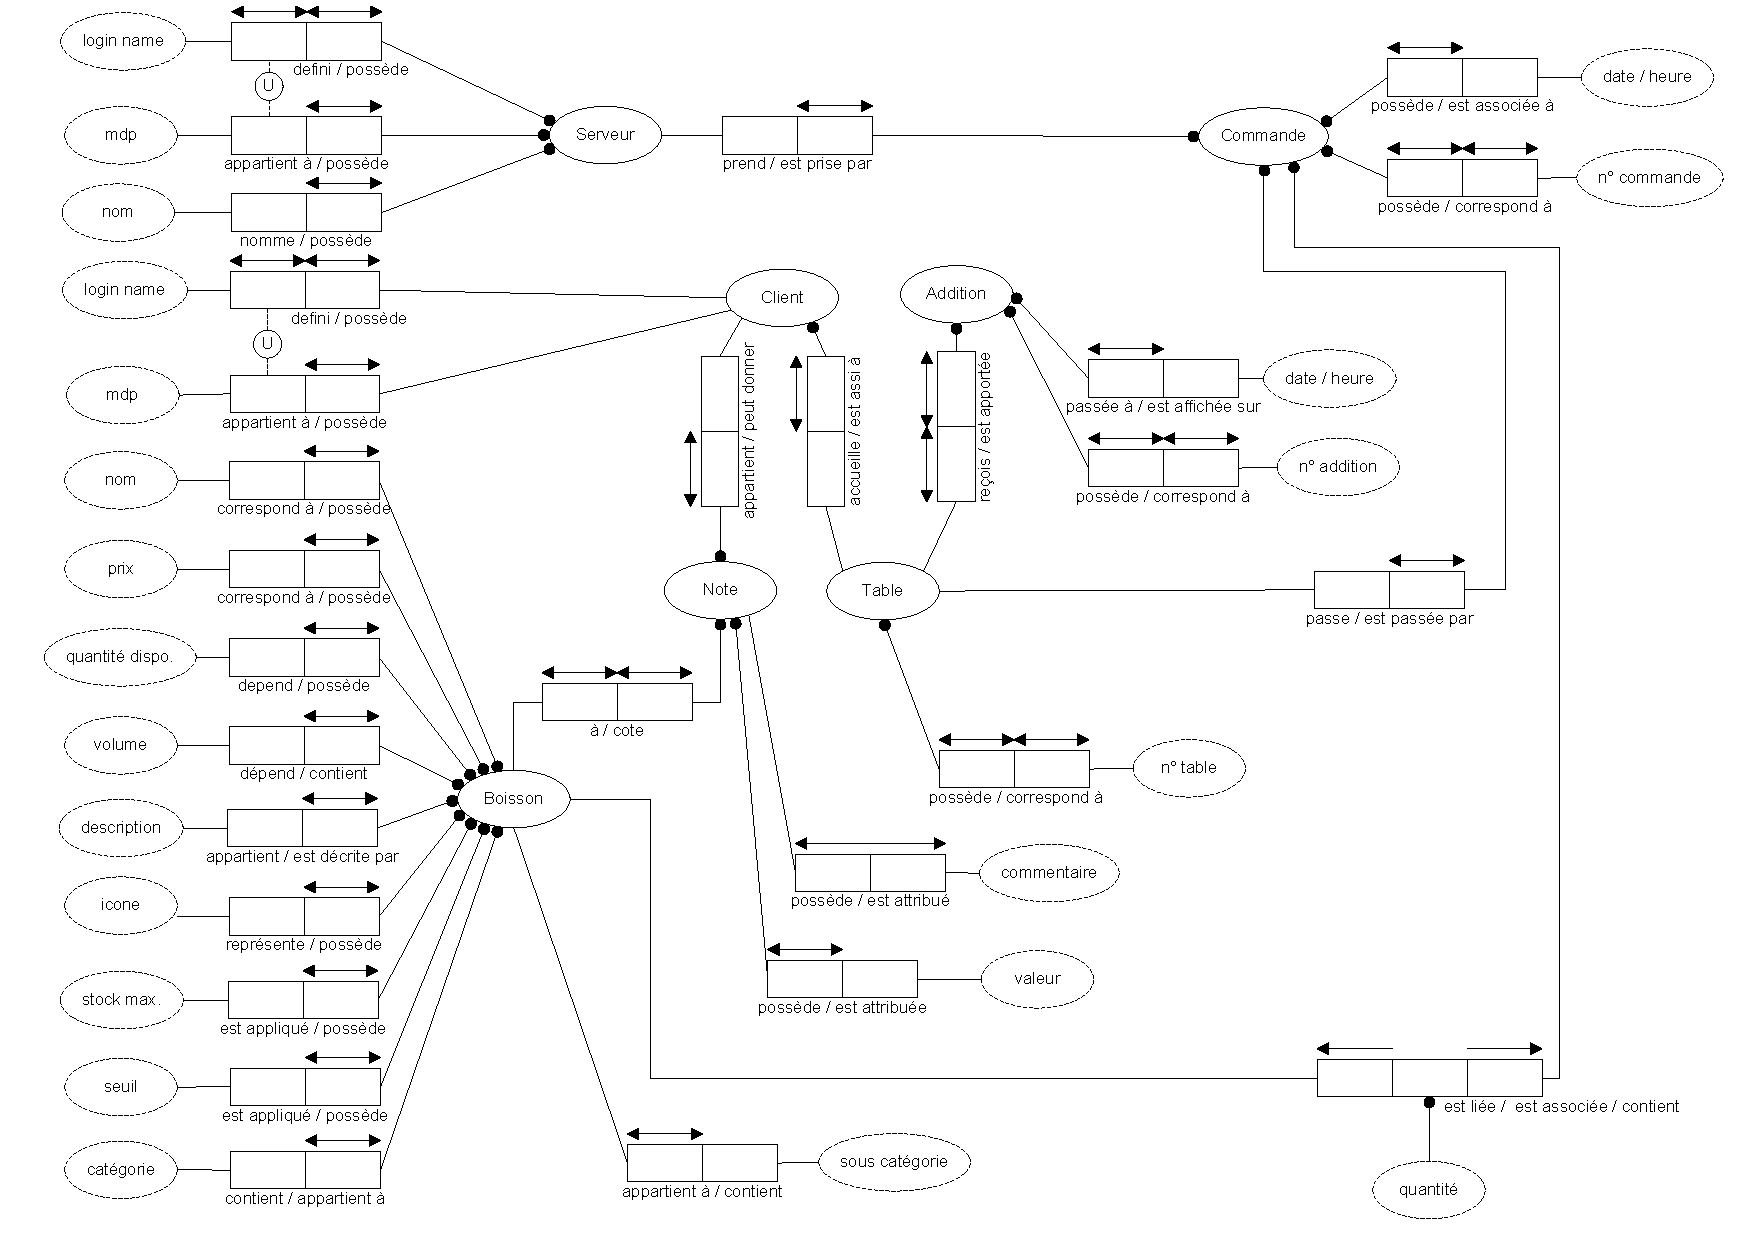
\includegraphics[scale=0.67]{img/orm.pdf}}

\section{Population}
\label{sec:population}
\rotatebox{90}{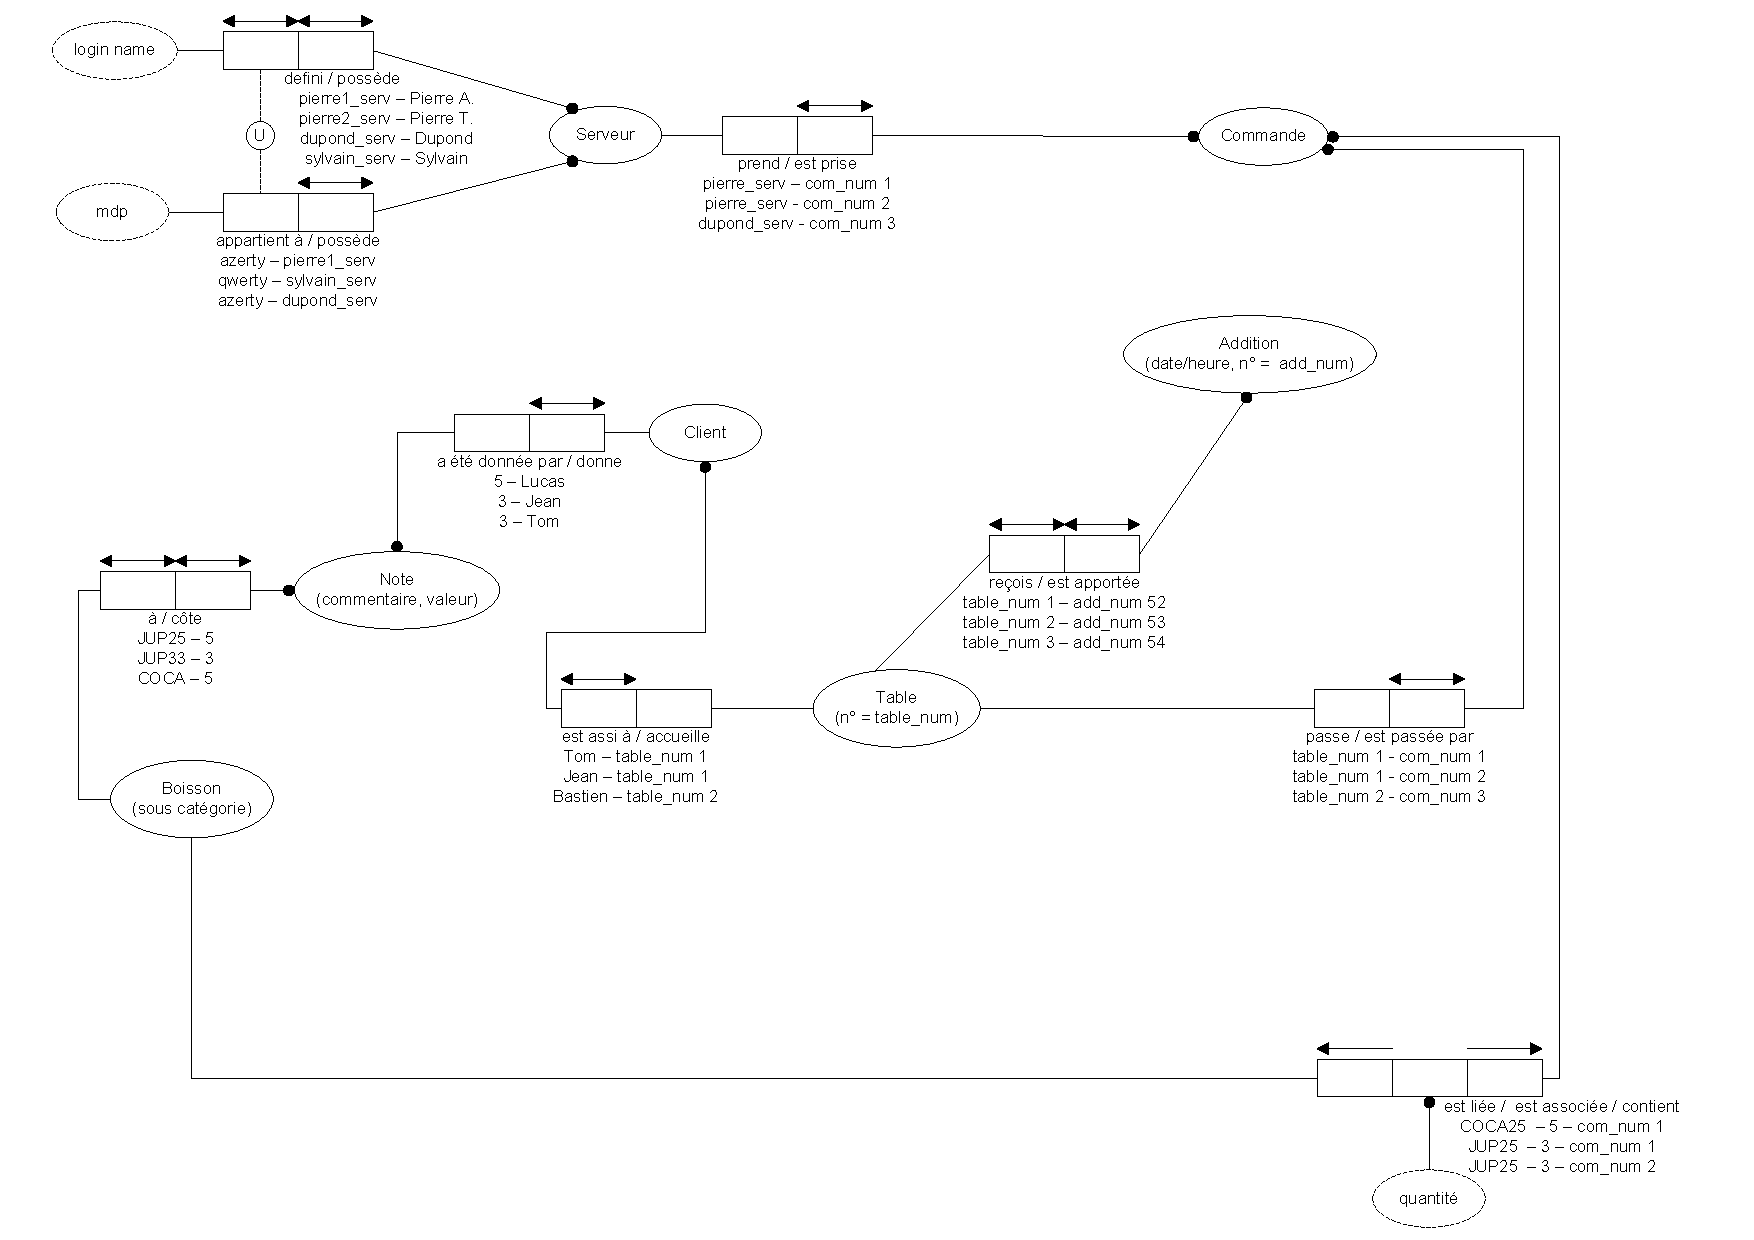
\includegraphics[scale=0.67]{img/population.pdf}}

\section{Structure de la BDD}
% TODO
\section{Requête sur la BDD}
% TODO
\end{document}